
\chapter{Esquema Detallado De Datos Y ETL}
\label{app:data-structures}

Este apéndice reúne el detalle estructural de las tablas intermedias y finales generadas por el pipeline de datos. Su objetivo no es introducir lógica nueva, sino dejar trazabilidad precisa sobre qué base crea cada etapa del ETL y cuál es el detalle de sus campos en \texttt{Read Raw Step}, \texttt{Merge Raw Step}, \texttt{Product Split Step}, \texttt{Underlying Step} y \texttt{Volatility Step}; las Figuras~\ref{fig:db-structure-details-read-raw} a~\ref{fig:db-structure-details-volatility} presentan, por etapa, la base generada y la estructura de sus campos.

\begin{figure}[!htpb]
\centering
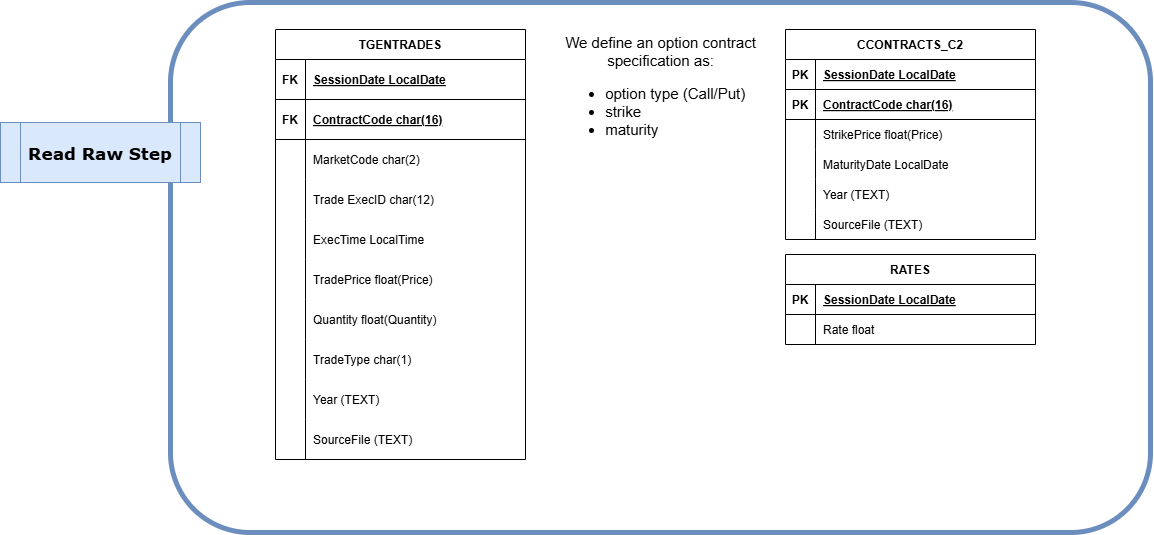
\includegraphics[width=0.98\textwidth,height=0.90\textheight,keepaspectratio]{../imgs/Read_Raw_step.drawio.png}%
\caption{\small Detalle estructural del ETL: \texttt{Read Raw Step}.}
\label{fig:db-structure-details-read-raw}
\end{figure}

\begin{figure}[!htpb]
\centering
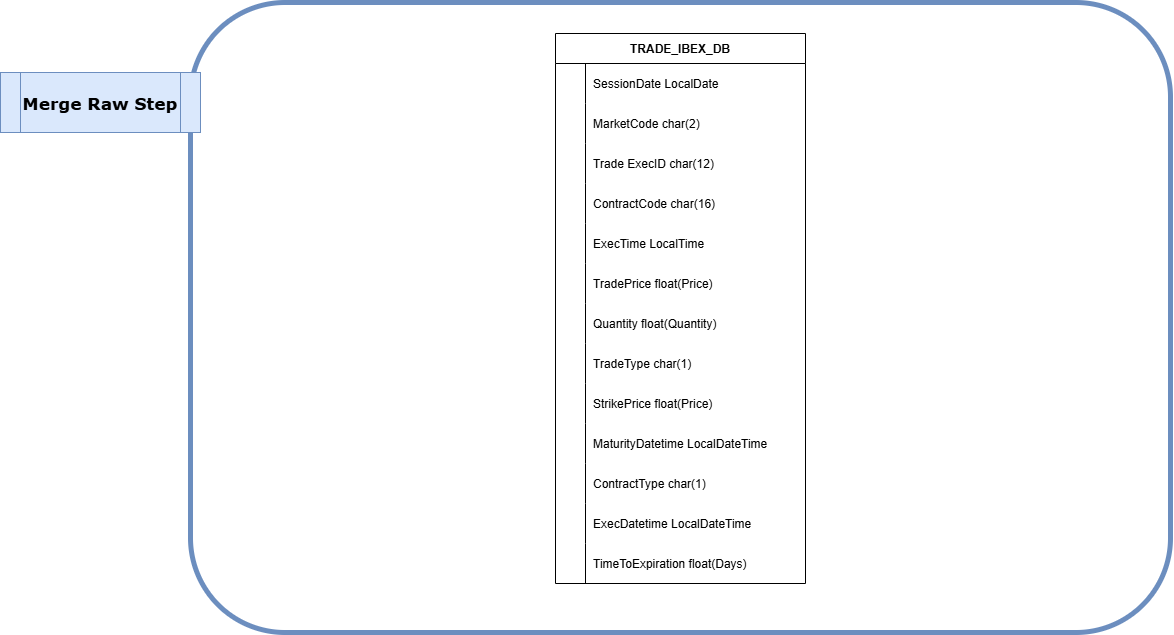
\includegraphics[width=0.98\textwidth,height=0.90\textheight,keepaspectratio]{../imgs/Merge_Raw_step.drawio.png}%
\caption{\small Detalle estructural del ETL: \texttt{Merge Raw Step}.}
\label{fig:db-structure-details-merge-raw}
\end{figure}

\begin{figure}[!htpb]
\centering
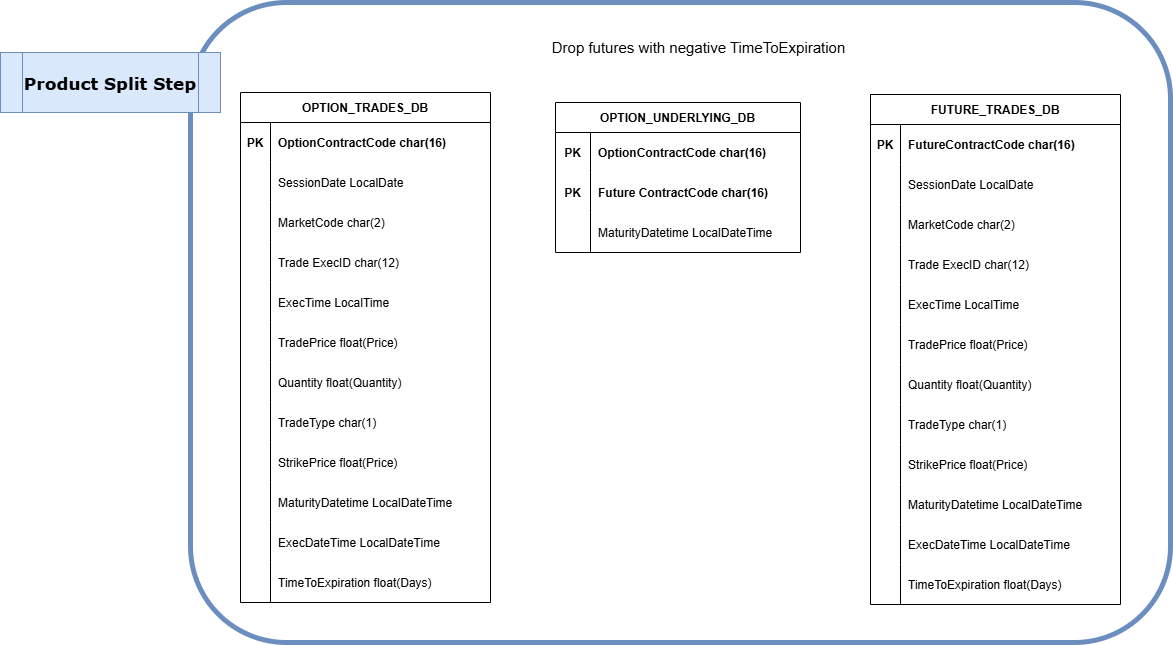
\includegraphics[width=0.98\textwidth,height=0.90\textheight,keepaspectratio]{../imgs/Product_Split_step.drawio.png}%
\caption{\small Detalle estructural del ETL: \texttt{Product Split Step}.}
\label{fig:db-structure-details-product-split}
\end{figure}

\begin{figure}[!htpb]
\centering
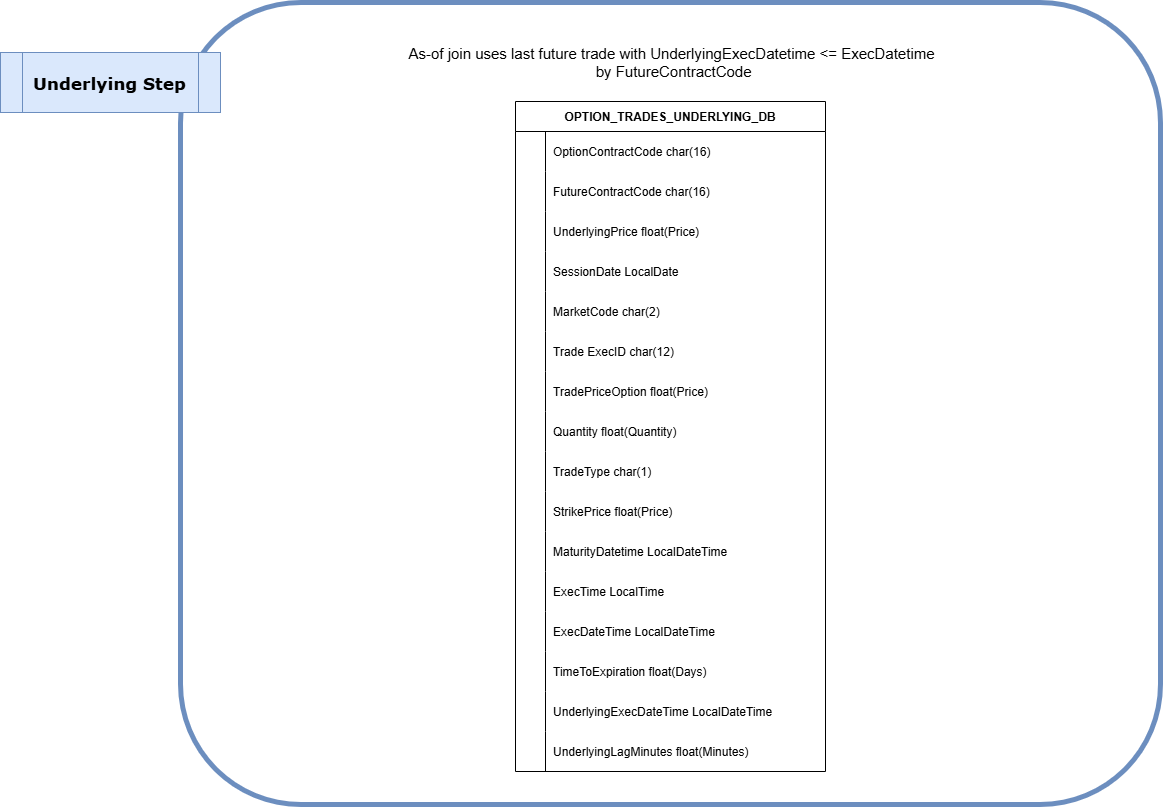
\includegraphics[width=0.98\textwidth,height=0.90\textheight,keepaspectratio]{../imgs/Underlying_step.drawio.png}%
\caption{\small Detalle estructural del ETL: \texttt{Underlying Step}.}
\label{fig:db-structure-details-underlying}
\end{figure}

\begin{figure}[!htpb]
\centering
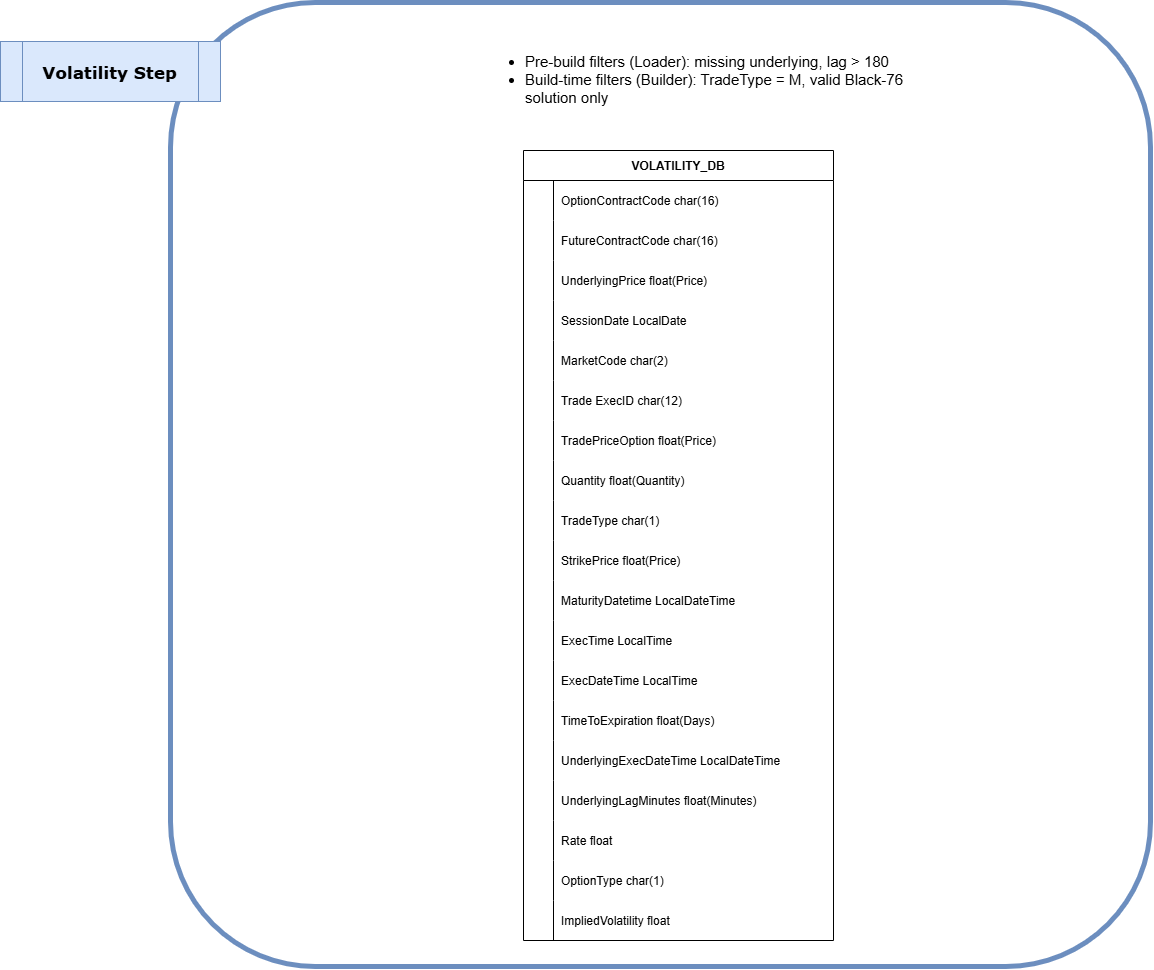
\includegraphics[width=0.98\textwidth,height=0.90\textheight,keepaspectratio]{../imgs/Volatility_step.drawio.png}%
\caption{\small Detalle estructural del ETL: \texttt{Volatility Step}.}
\label{fig:db-structure-details-volatility}
\end{figure}
